\section{Experimentelles Vorgehen}
In der Versuchsdurchführung soll in jeweils drei Versuchsdurchläufen der Gefrierpunkt von destilliertem Wasser sowie von einer Salzlösung (in diesem Fall: $NaNO_3$) festgestellt werden. Zusätzlich soll der Temperaturverlauf des Wassers/der Lösung alle 5 Sekunden protokolliert werden. Die Temperatur soll mithilfe eines Thermistors bestimmt werden, der im Anschluss kalibriert wird. Wie in Abb. \ref{fig:aufbau} dargestellt, wird das Reagenzglas mit der Testflüssigkeit in ein Kältebad mit etwa $\unit[-6]{^\circ C}$ gegeben. Sobald sich der Transistor wie in der Abbildung skizziert in der Lösung befinden, wird mit der Messung begonnen. Während der Messung wird mithilfe der Rührer sowohl das Kältebad als auch die Testflüssigkeit durchmischt, um eine homogene Temperaturverteilung zu gewährleisten. Ist der Widerstand (also die Temperatur) für längere Zeit konstant, ist der Gefrierpunkt erreicht worden, welcher durch die anschließende Kalibrierung ermittelt werden kann.\\
Das Kältebad wird auf $\unit[-6]{^\circ C}$ gebracht, indem der Gefrierpunkt des Wassers mithilfe von Streusalz ($NaCl$) erniedrigt wird. Anschließend wird das Gemisch mithilfe von Eis auf die entsprechende Temperatur gebracht. Die Temperatur wird hierbei mit einem normalen Digitalthermometer gemessen.


\begin{figure}
\begin{center}
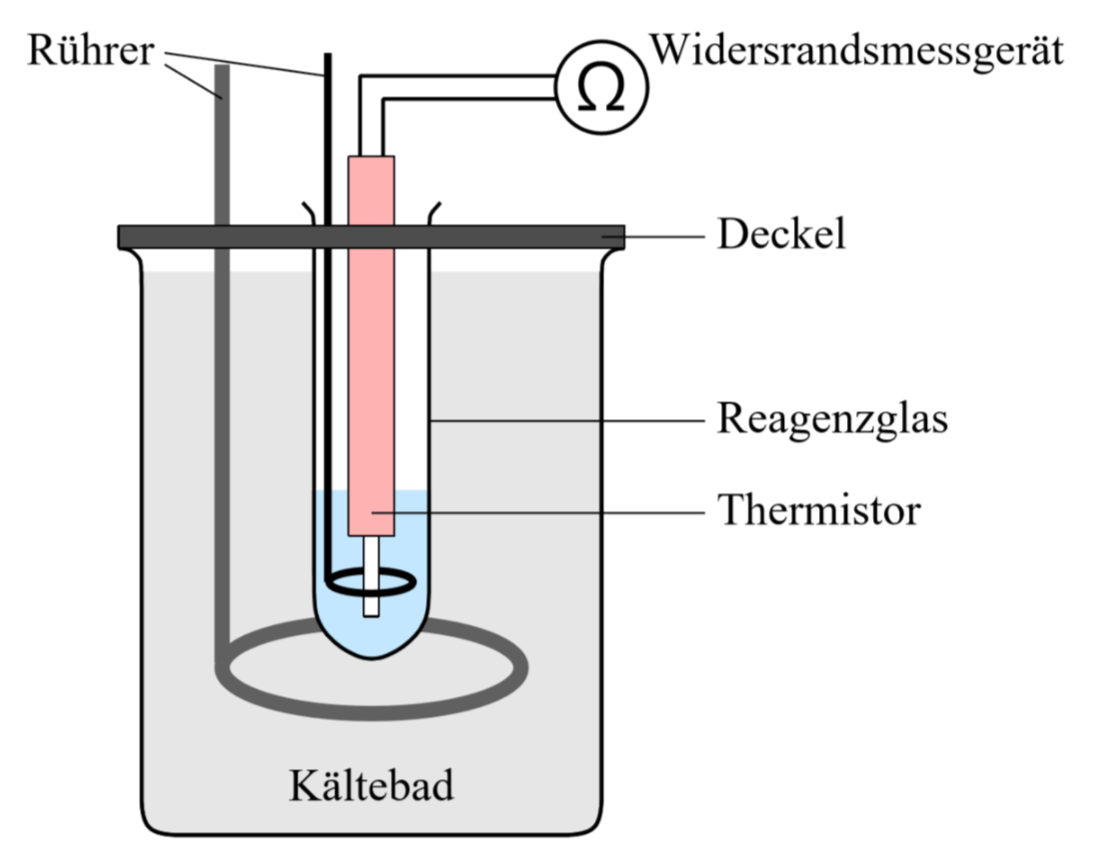
\includegraphics[scale=0.5]{Bilder/Versuchsaufbau.png}
\caption{Versuchsaufbau}
\label{fig:aufbau}
\end{center}
\end{figure}